\section{Projected Results}
\subsection{Kinematic Coverage}
\begin{figure}[!ht]
 \begin{center}
     \subfloat[w/o PRD]{
      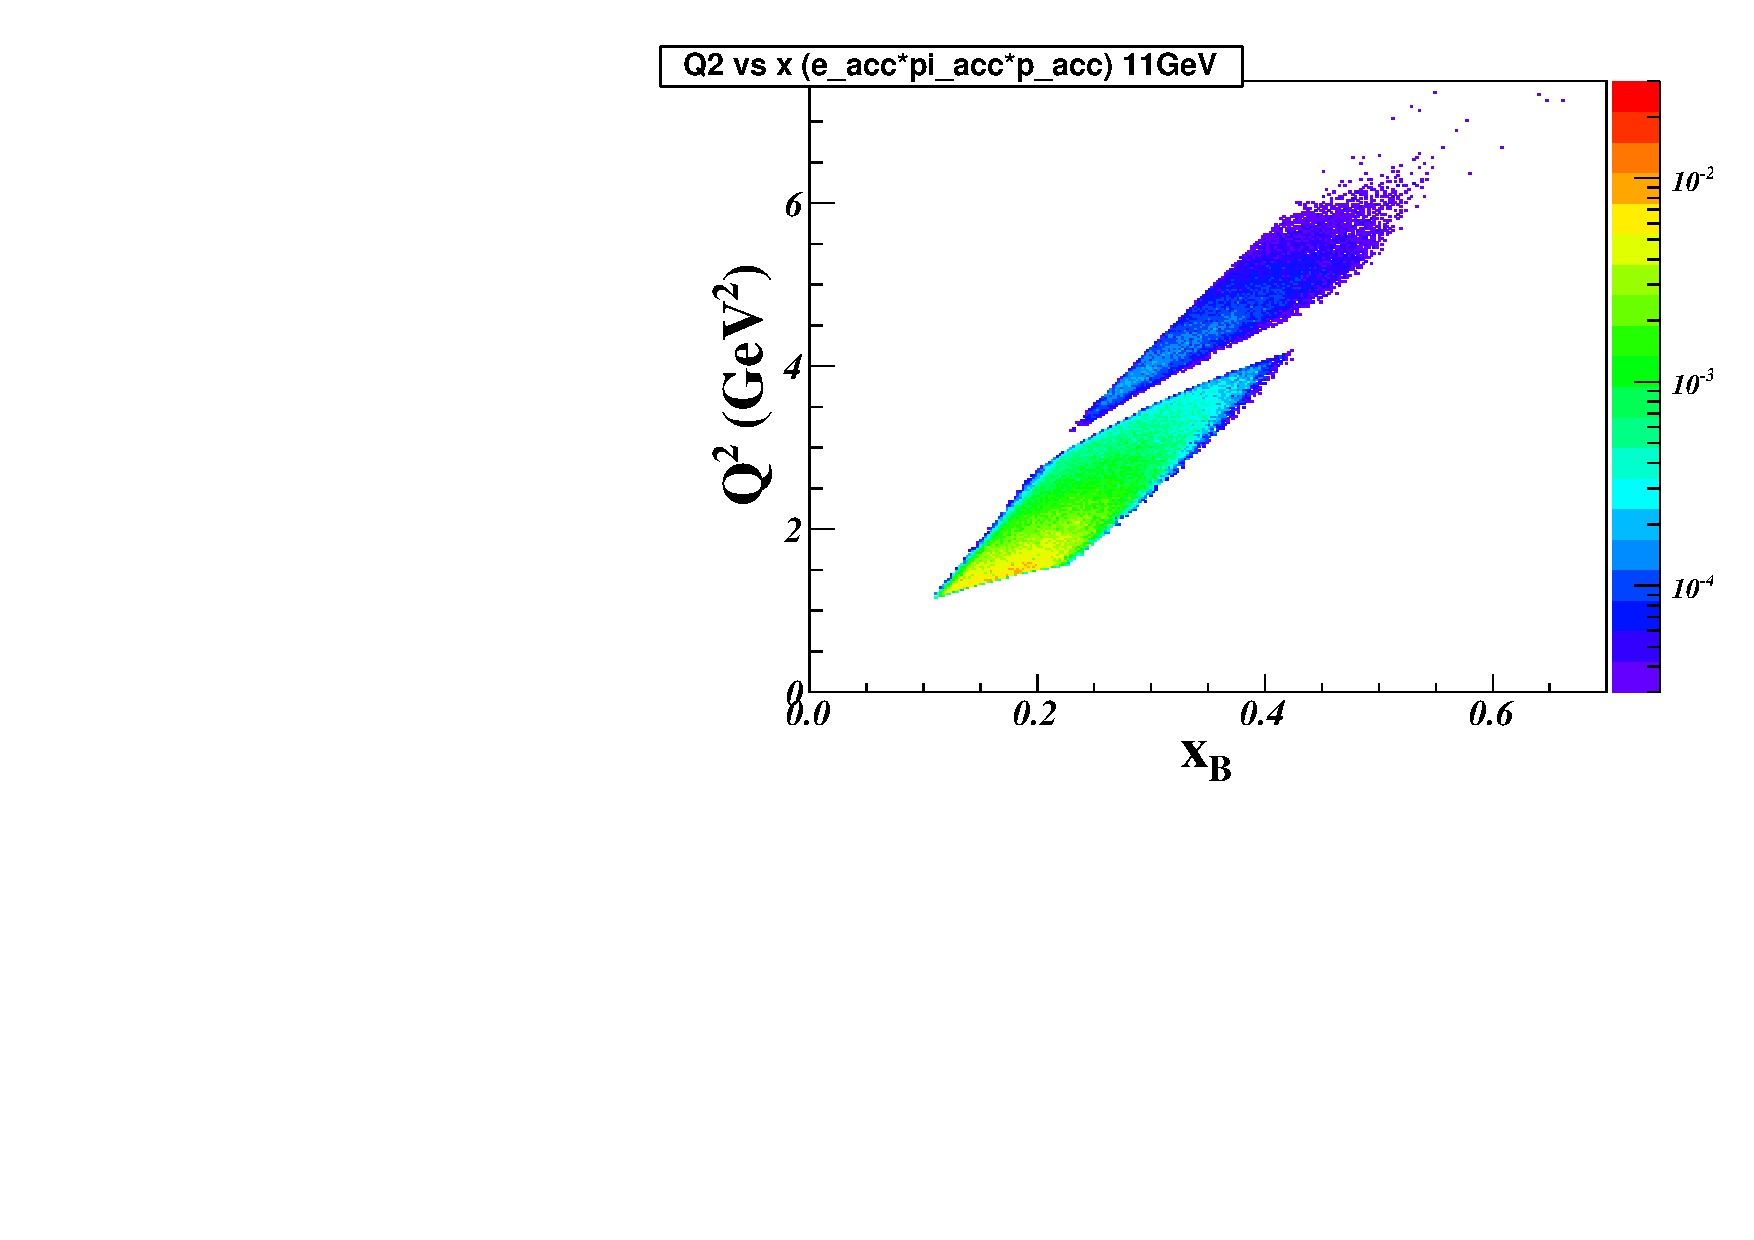
\includegraphics[type=pdf,
        ext=.pdf,read=.pdf,width=0.35\textwidth]{./figures//E11_Q2_x_epip_prd}
    }
     \subfloat[w PRD]{
      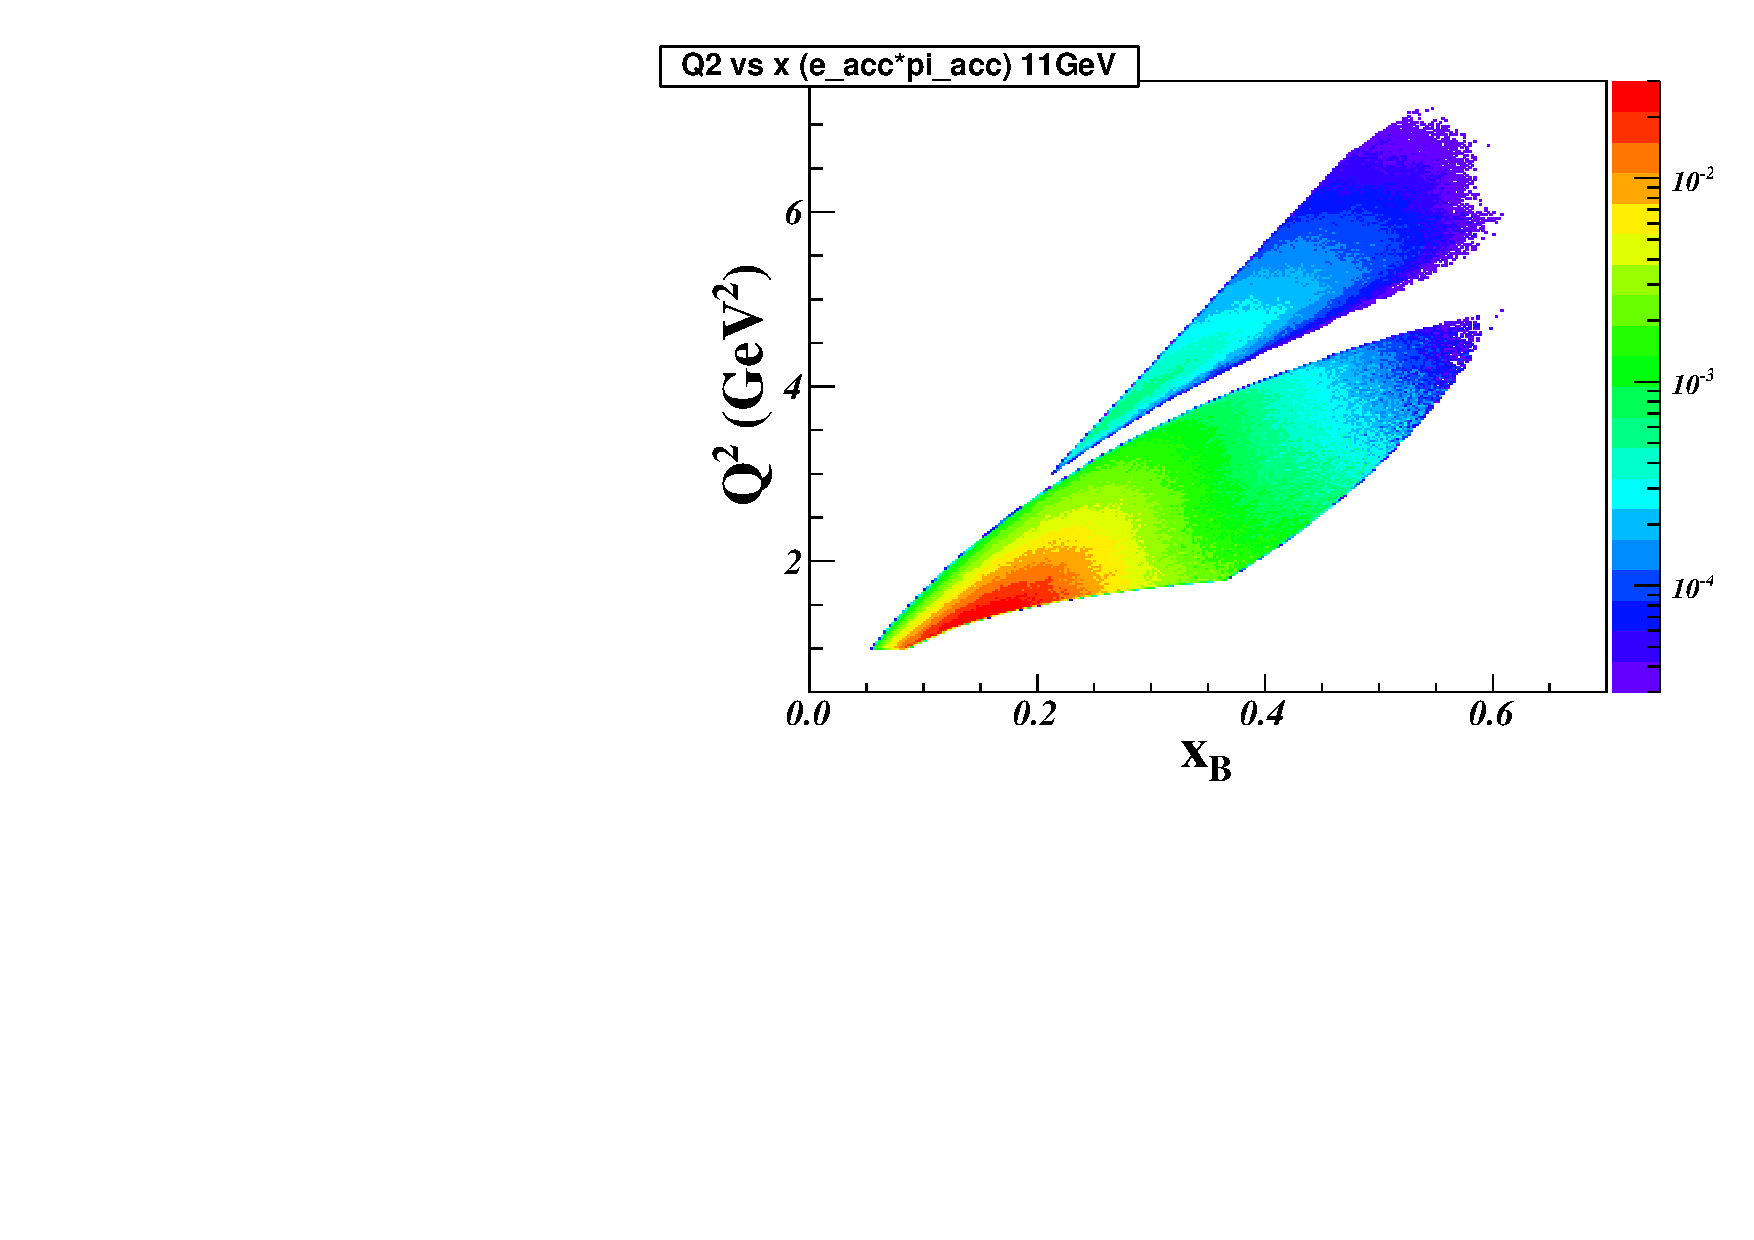
\includegraphics[type=pdf,
        ext=.pdf,read=.pdf,width=0.35\textwidth]{./figures/E11_Q2_x_epip}
    }    
 \caption[The kinematic coverage at different acceptances.]{\footnotesize{The
     kinematic coverage at different acceptances at 11~GeV. The left plot
     shows the coverage with proton detection by existing SoLID
     detectors, while the right  plot
     shows the coverage when detecting all recoil protons with an additional proton detector. Colors correspond to rates (Hz) in log scale.}}
  \label{kin_cor}
  \end{center}
\end{figure}

\begin{figure}[!ht]
 \begin{center}
       \subfloat[w/o PRD]{
      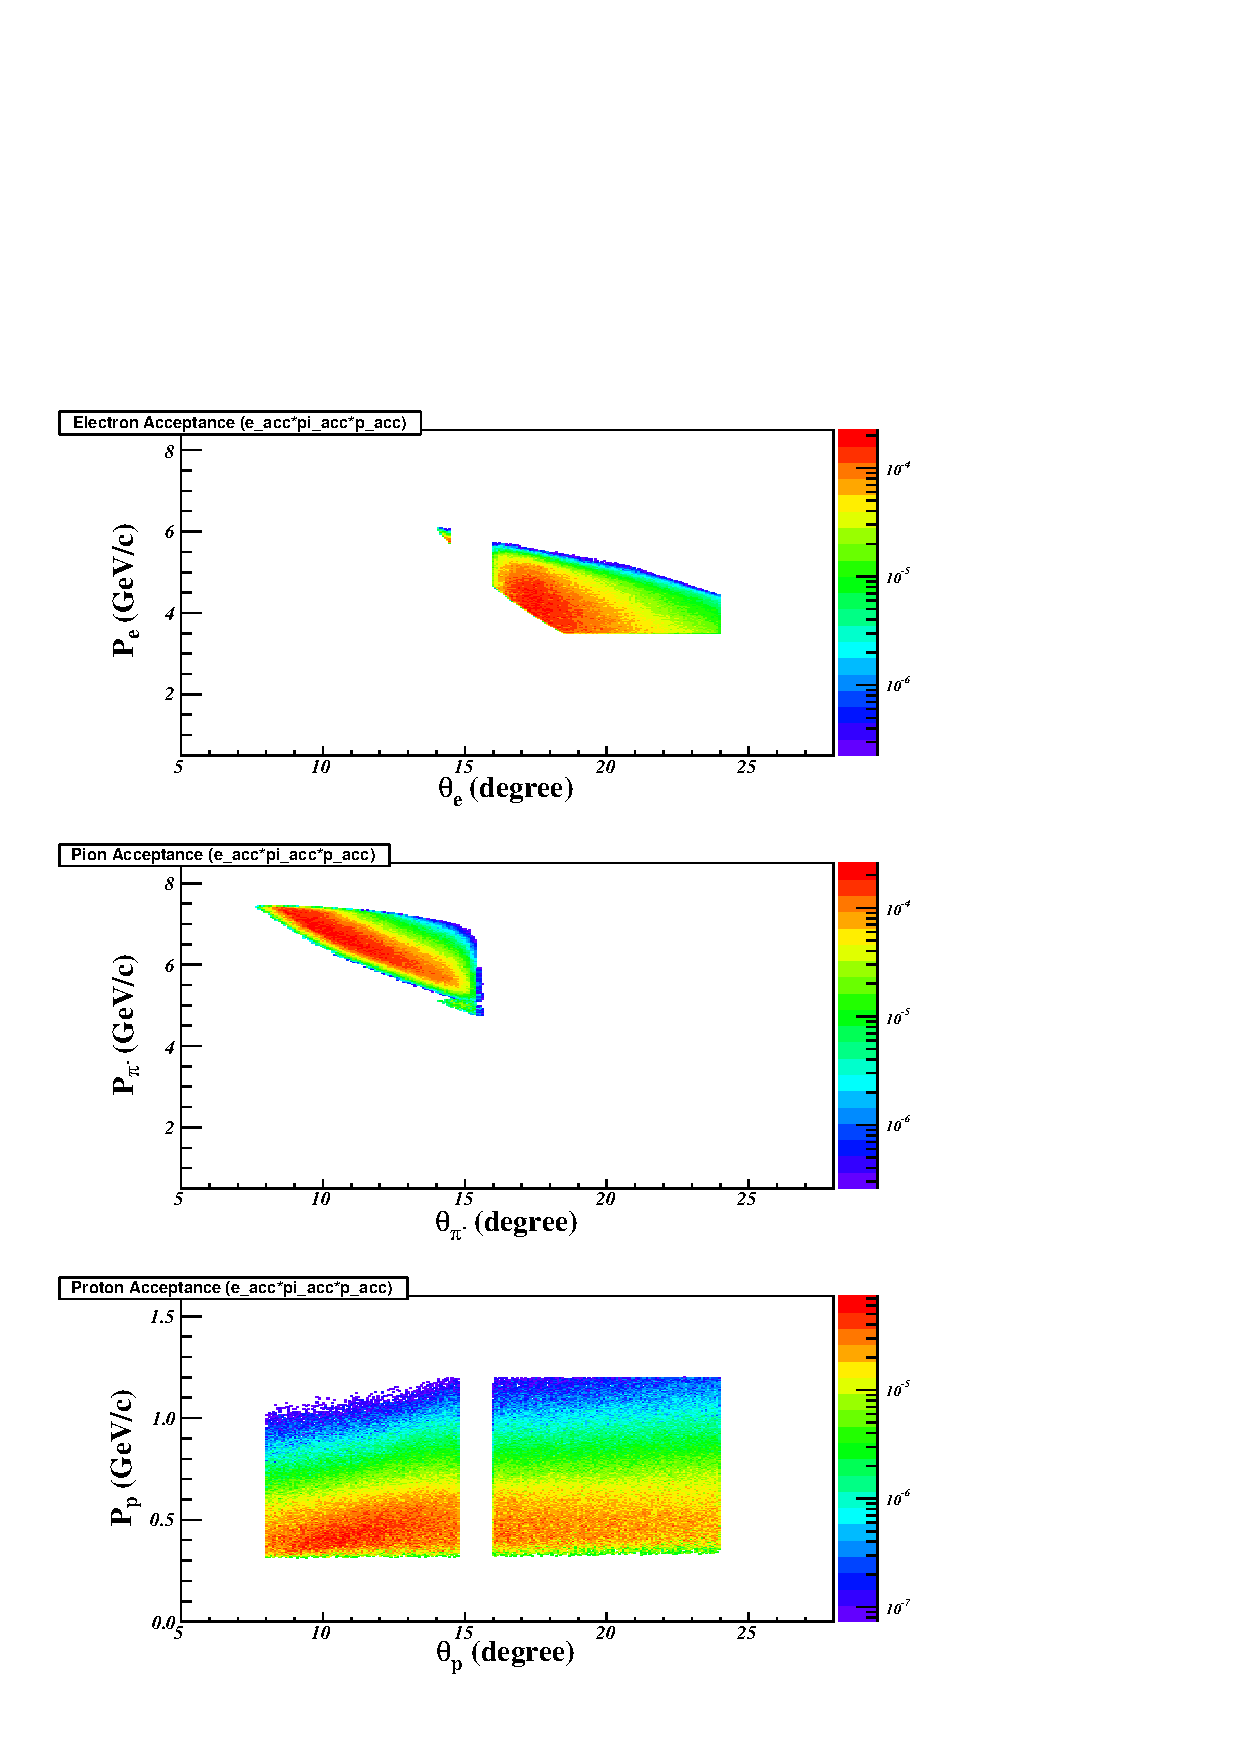
\includegraphics[type=pdf,
        ext=.pdf,read=.pdf,width=0.35\textwidth]{./figures/E11_acc_epip_Q2gt4}
    }
  \subfloat[w/ PRD]{
      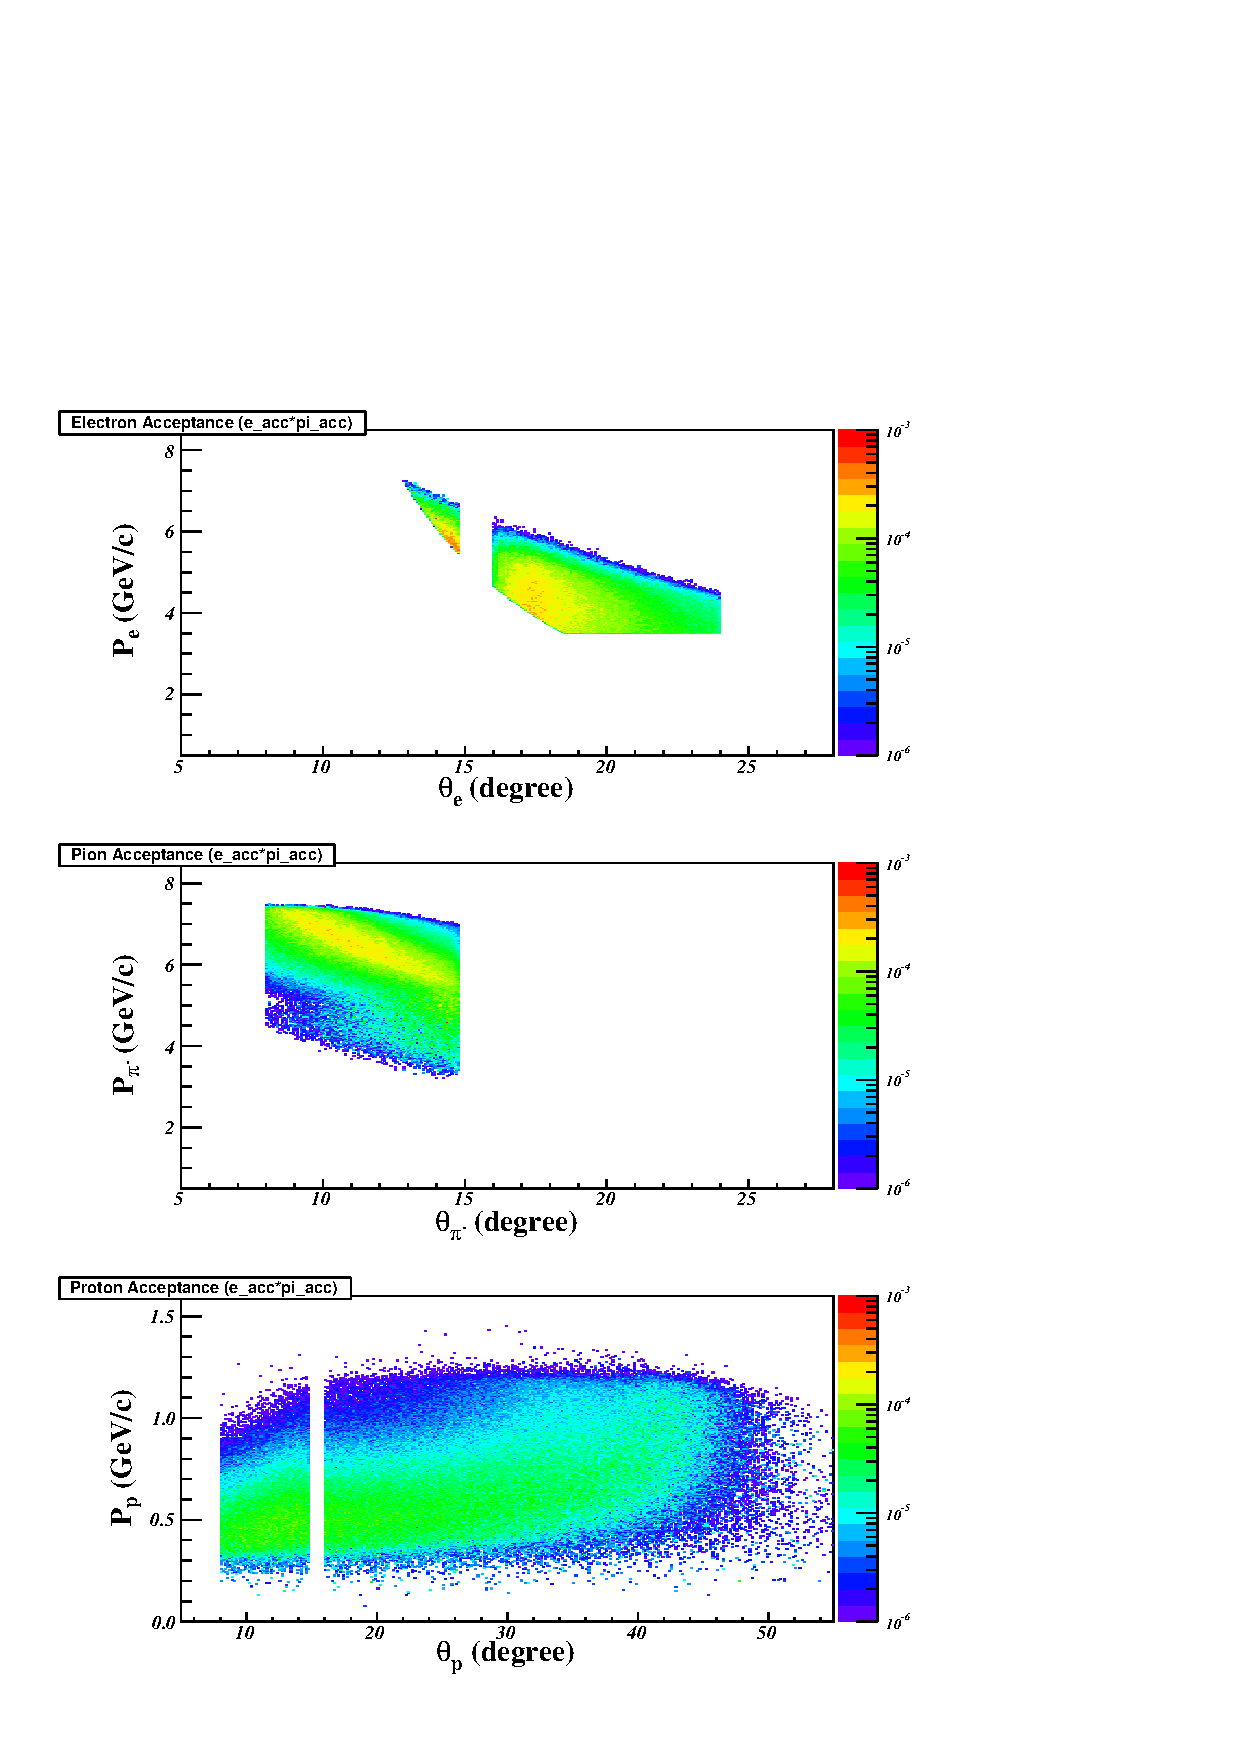
\includegraphics[type=pdf,
        ext=.pdf,read=.pdf,width=0.35\textwidth]{./figures/E11_acc_epi_Q2gt4}
    }  
   \caption[The acceptance of the momenta and scattering angles for electrons,
     $\pi^{-}$ and protons]{\footnotesize{The acceptance of the momenta and
       polar angles w/o or w/ the PRD. In each panel, the top, middle and
       bottom plots are for electrons, $\pi^{-}$ and protons, respectively. A
       cut of $\mathrm{Q^{2}>4~GeV^{2}}$ is applied. Colors correspond to rates
       (Hz) in log scale.}}
  \label{p_theta}
  \end{center}
\end{figure}
The kinematic coverage in $Q^{2}$ vs. $x_{B}$ is shown in Fig.~\ref{kin_cor},
where two proton detection cases were given: $(a)$ by using only the SoLID
detectors to detect protons at small angles ($8^{\circ}\sim24^{\circ}$) and
adding a new proton recoil detector to detect the rest of the recoil protons at
larger angle ($24^{\circ}\sim50^{\circ}$), or $(b)$ by only using only the 
SoLID detectors. These distributions were weighted by the DEMP unpolarized
cross sections and the SoLID acceptance obtained from the GEANT4 simulation
with the SoLID-SIDIS configuration. As shown in these plots, the range of
$Q^{2}$ is from 1.0~GeV$^{2}$ to 8.0~GeV$^{2}$, $x_{B}$ goes from 0.1 up to
0.75.

Fig.~\ref{p_theta} shows the momentum and angular acceptance of electrons,
$\pi^{-}$ and protons which form the DEMP events and can be detected with the
SoLID detectors and (or) with the new PRD.  A cut of $Q^{2}>$4~GeV$^{2}$
is applied since this is the region of greatest physics itnerest.  The recoil
protons shown in Fig.~\ref{p_theta} have low momenta ranging from 0.3~GeV/c up
to 1.2~GeV/c and their rates are distributed nearly uniformly in scattering
angle.

\subsection{Estimated Rates}
\begin{table}[!ht]
\centering
\begin{tabular}{|c|c|c|}
 \hline
  1$<Q^{2}<$4~GeV$^{2}$ & $Q^{2}>$4~GeV$^{2}$ & Total\\
 \hline
\multicolumn{3}{|c|}{DEMP: $\vec{n}(e,e'\pi^{-}p)$ Triple-Coincidence (Hz)}\\
 \hline
 17.79 (0.22)   &  0.53 (0.31) & 26.45 (7.66)   \\
 \hline
\multicolumn{3}{|c|}{SIDIS: $\vec{n}(e,e'\pi^{-})X$ Double-Coincidence (Hz)}\\
 \hline
        1388.85 & 35.77        & 1424.62   \\
 \hline
\end{tabular}
\caption[Triple-Coincidence rates for
  neutron-DEMP]{\footnotesize{Triple-Coincidence rates for DEMP events compared
    with the SIDIS rates. Numbers in brackets are the DEMP rates with only
    detecting protons using only the SoLID detectors. The online production
    trigger will be the SIDIS double-coincidence trigger of which rates are
    also given.}}
\label{rate_table}
\end{table} 
Table~\ref{rate_table} lists the triple-coincidence rate of the DEMP
events. The rates were calculated with the simulated events weighted by the
target luminosity, the SoLID acceptances and unpolarized cross sections. The
rates are not corrected by the beam and target polarization, target dilution
and so on. The total integrated physics rate is estimated to be around 26~Hz at
11~GeV, or 0.53 Hz at $Q^{2}>$4~GeV$^{2}$. If only using only the 
SoLID detectors to detect protons, the rate drops to 0.31 Hz at
$Q^{2}>$4~GeV$^{2}$.  For comparison, the table also gives the SIDIS rate
which will be the online production trigger rates and is the main background of
the DEMP events.

\subsection{Asymmetry Projections}
\begin{figure}[!ht]
 \begin{center}
       \subfloat[w/o PRD]{
      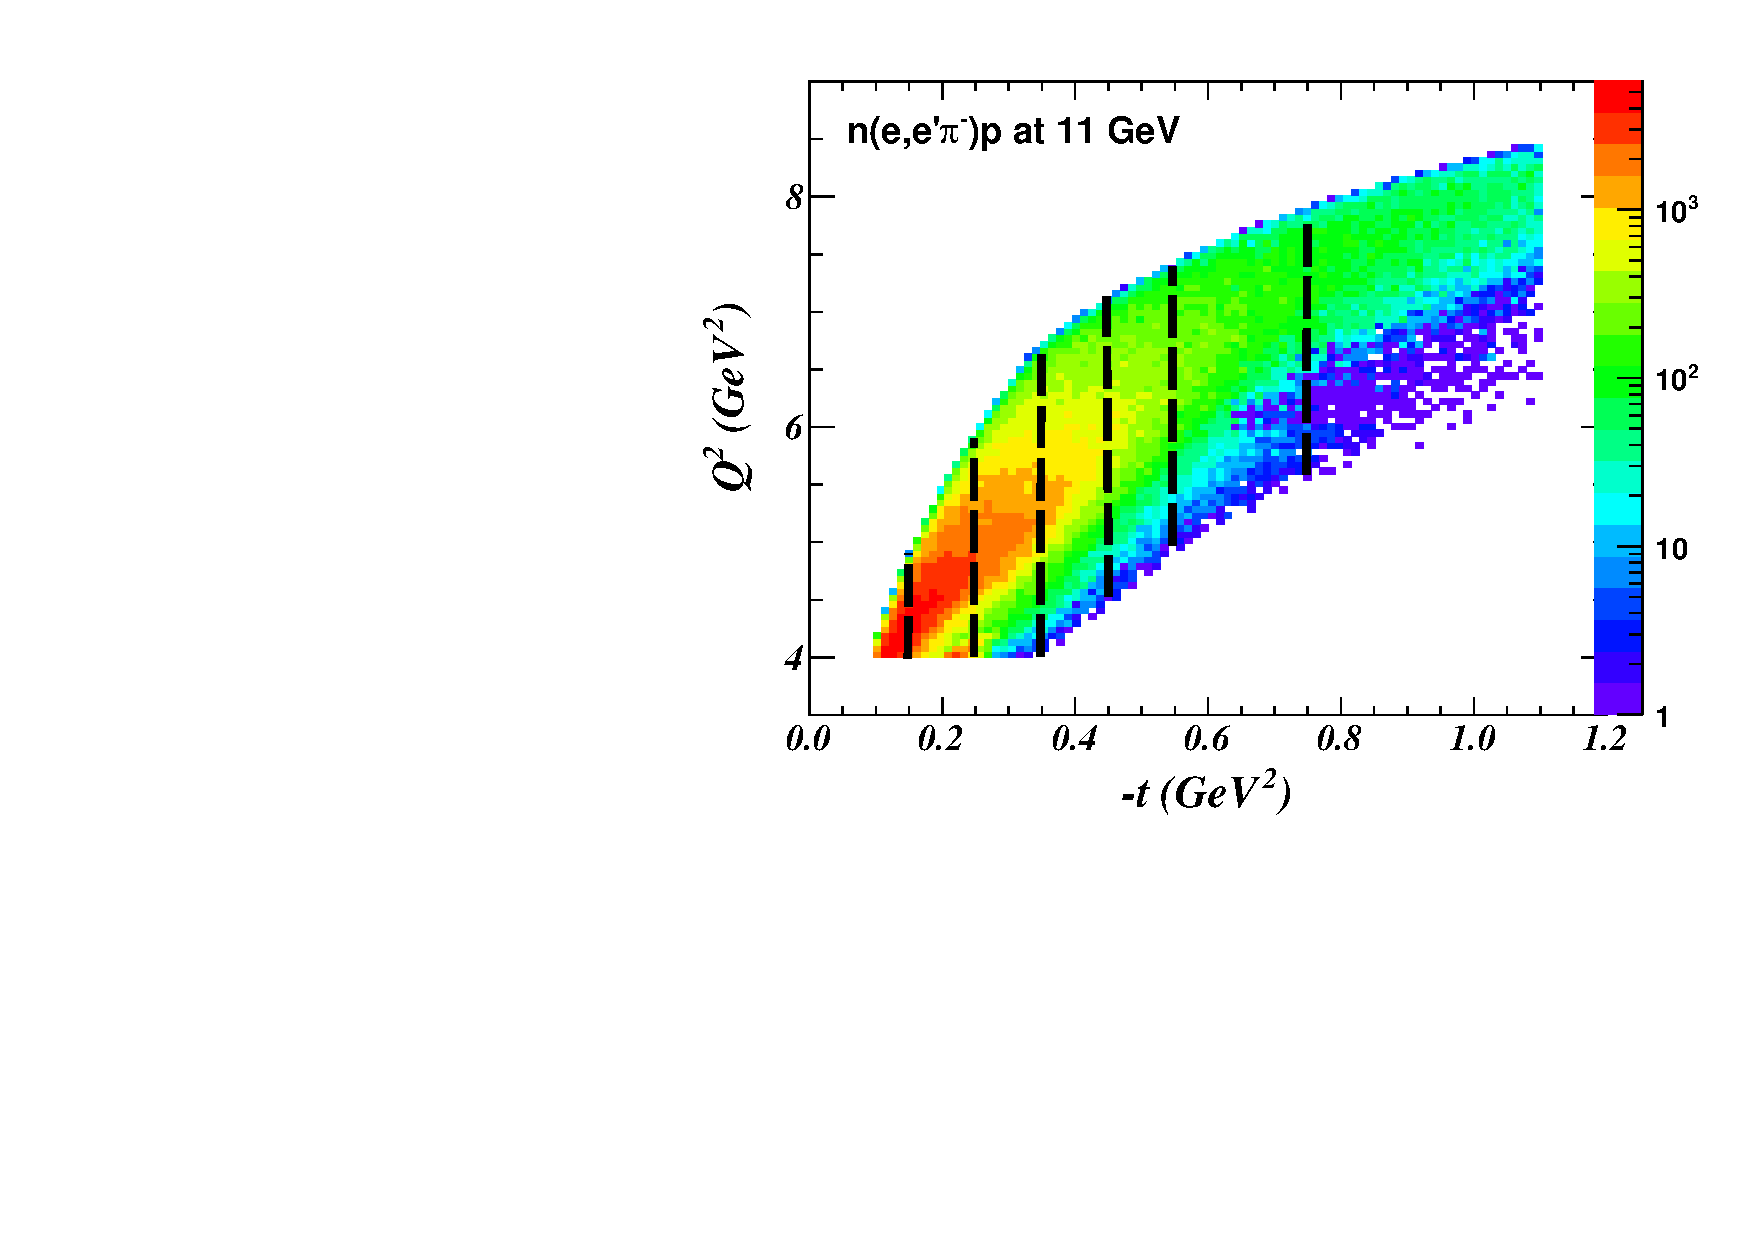
\includegraphics[type=pdf,
        ext=.pdf,read=.pdf,width=0.5\textwidth]{./figures/E11_Q2_t_bin} }
        \subfloat[w/ PRD]{
      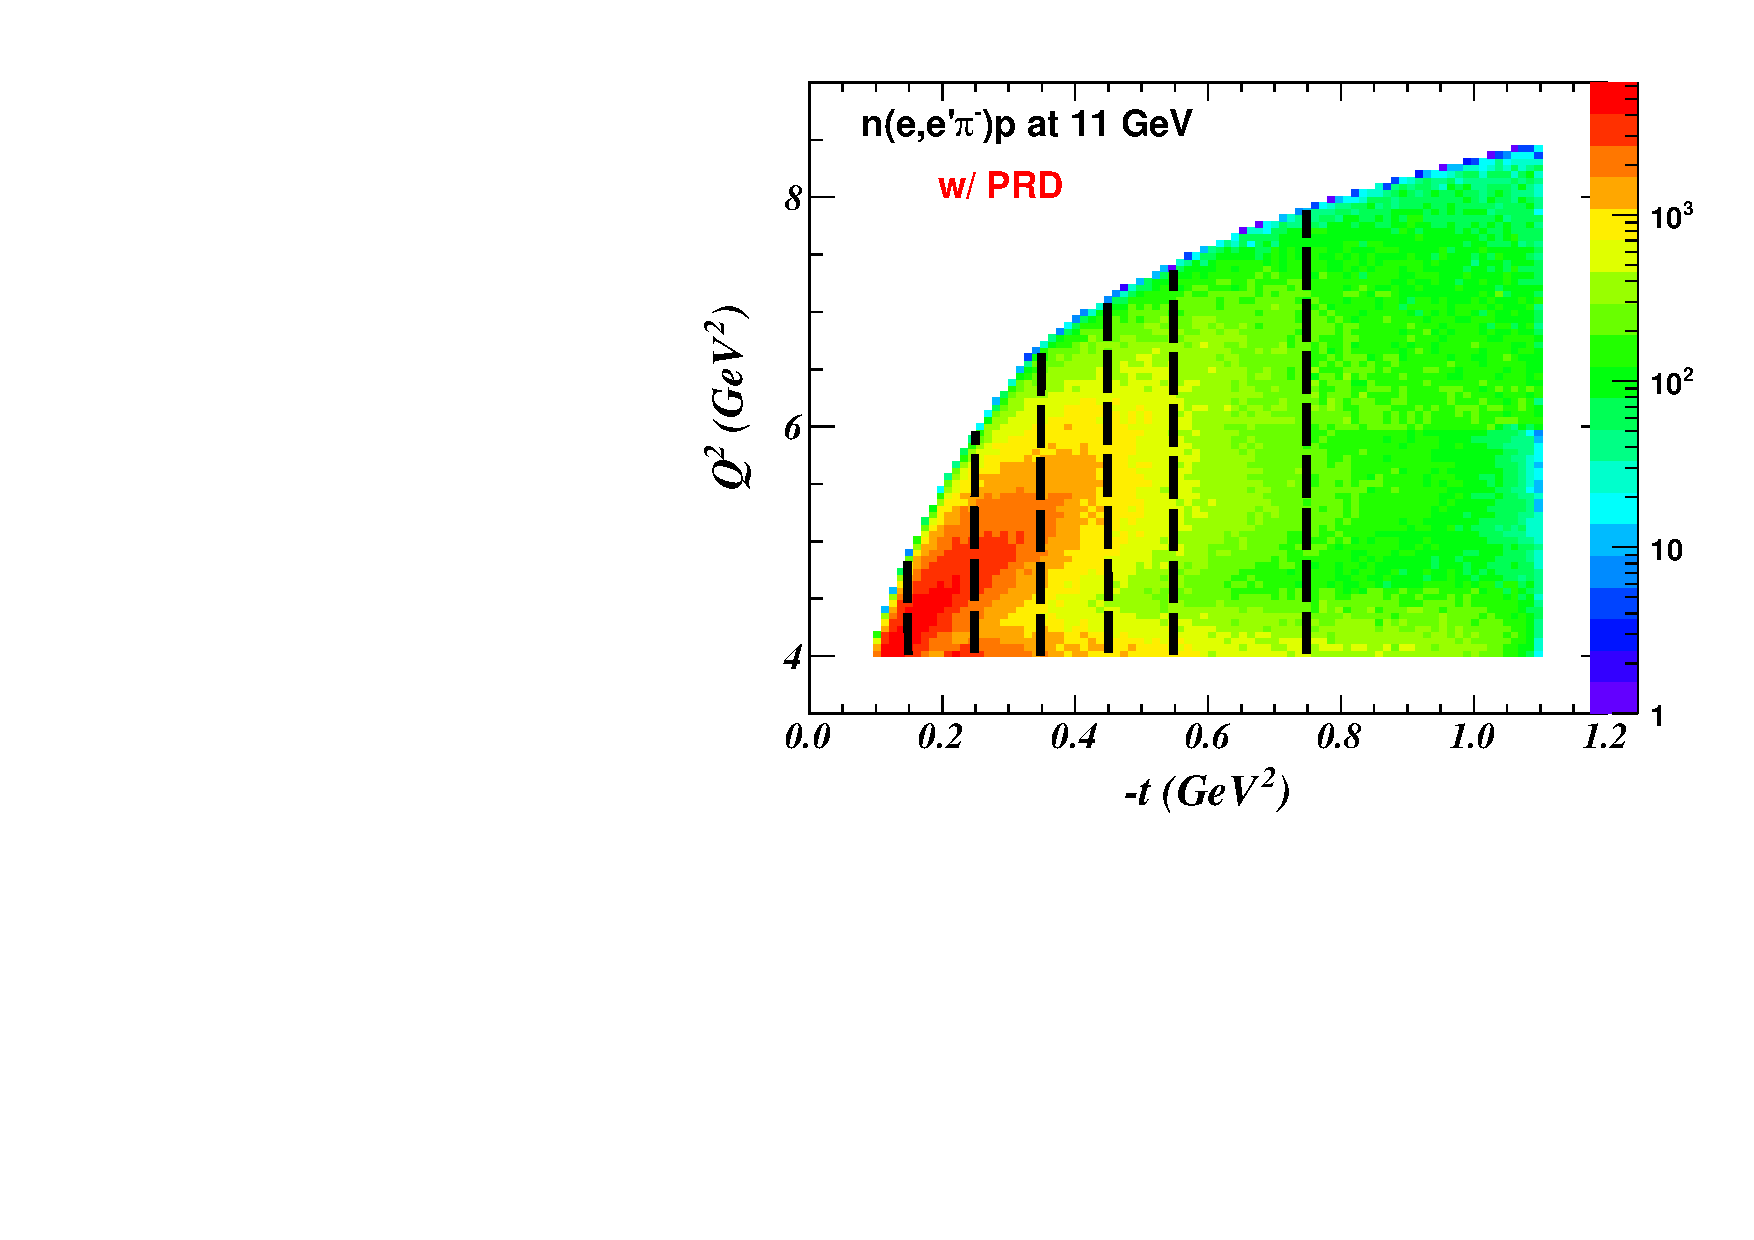
\includegraphics[type=pdf,
        ext=.pdf,read=.pdf,width=0.5\textwidth]{./figures/E11_Q2_t_bin_prd} }
   \caption[$Q^{2}$ vs. $-t$]{\footnotesize{$Q^{2}$ vs. $-t$ where the black
       dash lines specify the boundaries of 7 $-t$ bins. The color panel
       indicates the raw counts with 48 days of beam time at 11~GeV.}}
  \label{Q2_t_bin}
  \end{center}
\end{figure}
The proposed experiment will run in parallel with E12-10-006 which has already
been approved to run 48 days at $E_{0}$=11~GeV.  As shown in
Fig.~\ref{Q2_t_bin}, We defined 7 $-t$ bins of which the the boundaries are
defined by the array:
 \begin{equation}
   -t[8] = [0.0, 0.15, 0.25, 0.35, 0.45, 0.55, 0.75, 1.10]~~~~(in~\mathrm{GeV^{2}})
 \end{equation}
The number of events ($N_{i}$) in the $i$th bin is calculated from the total
simulated events after applying cuts on important kinematic variables,
e.g. $Q^{2}>$4~GeV$^{2}$, $W>$2~GeV, 0.55$<\epsilon<$0.75 and
$-t_{min}<-t<-t_{max}$. As shown in Eq.~\ref{ncount}, each event surviving the
cuts is then weighted by the unpolarized cross section, together with the
acceptance of the electron, pion and proton. $N_{i}$ is further corrected by
the phase-space factor ($PSF$) defined in the event generator, the total number
of randomly generated events ($N_{gen}$), beam-time ($T$), the target
luminosity ($L=10^{36}$~cm$^{-2}$s$^{-1}$), and the overall detector efficiency 
($\epsilon_{eff}$):
 \begin{equation}
     N_{i} = \bigl(\sum_{j\in i-bin} \sigma_{j}\cdot A^{e}_{j} \cdot
     A^{\pi^{-}}_{j} \cdot A^{p}_{j}\bigr) \cdot (PSF/N_{gen}) \cdot T \cdot L \cdot
     \epsilon_{eff},
     \label{ncount}
 \end{equation}
where $j$ is the $j$th event in the $i$th bin, $\sigma_{j}$ is the cross
section of the $j$th event. $A^{e(\pi^{-},p)}_{j}$ is the acceptance weight of the
electron (pion, proton) in this event. The detector efficiency,
$\epsilon_{eff}$, is approximately fixed at 85\% which was used in SIDIS
proposals. $N_{i}$ corresponds to the raw experimental count of electrons
scattering on neutrons in $\mathrm{^{3}He}$ before taking into account the
target polarization ($P\sim60\%$), the effective polarization of neutrons
($\eta_{n}\sim0.865$), and the dilution effect from other reaction channels
when electrons scattering on $\mathrm{^{3}He}$ ($f \sim 0.9$). The statistical
error of the target single spin asymmetry ($A_{UT}$) in each bin can be given
as:
  \begin{equation}
    \delta A_{UT} = \frac{1}{P\cdot\eta_{n}\cdot f} \sqrt{\frac{1-(P\cdot
        <A_{UT}>)^{2}}{N^{+}_{i}+N^{-}_{i}}},
    \label{stat_err}
 \end{equation}
where $N^{+(-)}_{i}$ is the number of counts in each bin when the target
polarization is up (down), and we easily have $N_{i}=N^{+}_{i}+N^{-}_{i}$;
$<A_{UT}>$ is the average asymmetry in the bin, and experimentally, it can be
extracted as following:
\begin{equation}
   <A_{UT}> = \frac{1}{P\cdot\eta_{n}\cdot f} \frac{N^{+}-N^{-}}{N^{+}+N^{-}}.
   \label{asym_exp}
\end{equation}
In this projection study, $A_{UT}$ is predicted with a phenomenological model,
as discussed in Appendix-A. Because of not performing a L/T separation in this
experiment, the asymmetry should be corrected by another dilution factor which
is defined as:
\begin{equation}
  f_{L/T} =\frac{\epsilon\cdot\sigma_{L} }{\sigma_{T}+\epsilon\cdot\sigma_{L} },
\end{equation} 
where $\epsilon=1/(1+\frac{2\nu}{Q^{2}}\tan^{2}(\theta))$. Additional dilution
due to $\sigma_{TT}$ is assumed to be small.  Hence, $A_{UT} = f_{L/T}\cdot
A_{UT}^{model}$.

\begin{figure}[!ht]
 \begin{center}
         \subfloat[w/o PRD]{
               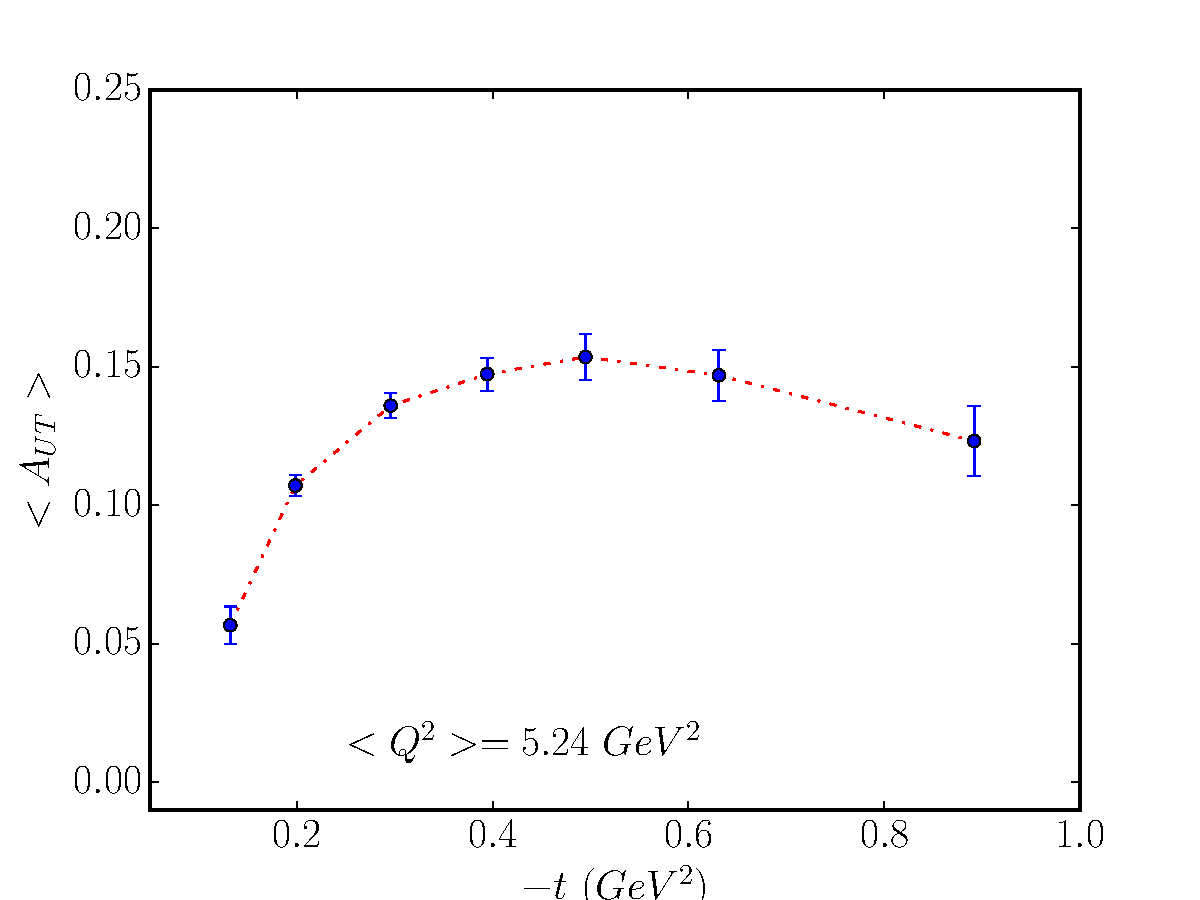
\includegraphics[type=pdf,
        ext=.pdf,read=.pdf,width=0.45\textwidth]{./figures/bin_asym_t} }
            \subfloat[w/ PRD]{
      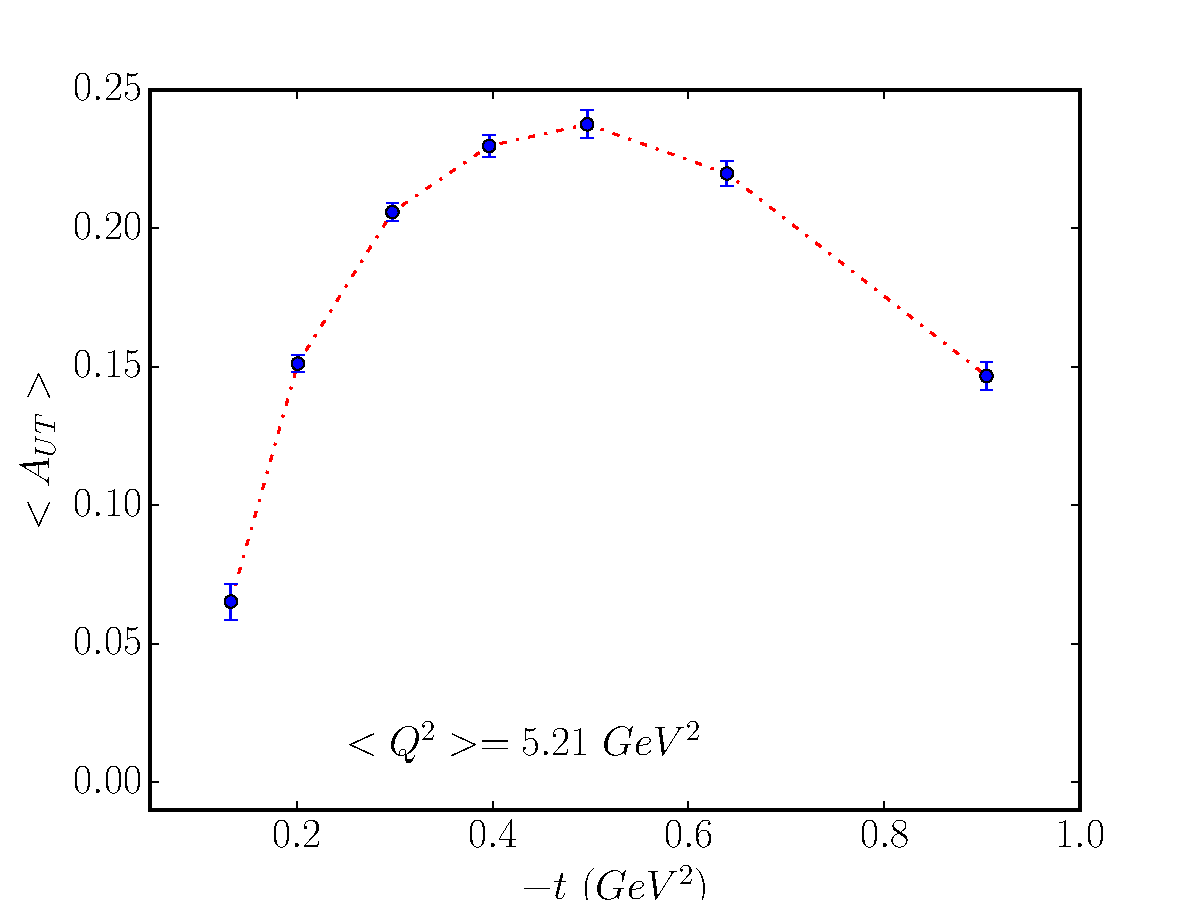
\includegraphics[type=pdf,
        ext=.pdf,read=.pdf,width=0.45\textwidth]{./figures/bin_asym_t_prd} }
      \caption{\footnotesize{Projection of target sing spin asymmetry
          ($A_{UT}$) in $-t$ binning for DEMP with transversely polarized
          $\mathrm{^{3}He}$ at $E_{0}$=11~GeV. The error bars are the projected
          statistical uncertainties defined in Eq.~\ref{stat_err}. The
          asymmetry value in each bin is predicted with the model given in Appendix-A and is diluted due to not separating the L/T
          contributions. The left plot shows the projection w/o a new proton
          recoil detector, while the right plot shows a better projected result
          with a new detector in addition. One can see the average asymmetries are also
          changed between two configurations and it is because the asymmetry
          strongly depends on $Q^{2}$ which changes w/ or w/o the PRD.}}
  \label{asym_t}
  \end{center}
\end{figure}
Fig.~\ref{asym_t} shows the distribution of $A_{UT}$ vs. $-t$ with projected
statistical errors discussed above. Compared with the existing HERMES results
(Fig.~\ref{fig:hermes_aut}), the new measurement could provide more precision
data to be directly compared with theoretical predictions. The detailed
information of each bin is listed in Table~\ref{asym_bin_table}.
	\begin{table}[!ht]
	\centering
	\begin{tabular}{|c|c|c|c|c|c|c|c|}
	  \hline
	w/o PRD   &  Bin\#1 & Bin\#2 & Bin\#3 & Bin\#4 & Bin\#5 & Bin\#6 & Bin\#7 \\
	\hline 
	    $<-t>$                &  0.13 & 0.20   & 0.30   & 0.39   & 0.49   & 0.63   & 0.89  \\
	   $<Q^{2}>$          & 4.22  & 4.67   & 5.23   & 5.78   & 6.26   & 6.81  & 7.59  \\
	   $<A_{UT}>$        &$5.67\times 10^{-2}$   & $1.07\times 10^{-1}$   & $1.36\times 10^{-1}$    & $1.47\times 10^{-1}$    & $1.54\times 10^{-1}$    & $1.47\times 10^{-1}$   & $1.23\times 10^{-1}$   \\
	   $\delta A_{UT}$  &  $6.76\times 10^{-3}$   & $3.73\times 10^{-3}$    &   $4.42\times 10^{-3}$  &  $5.92\times 10^{-3}$   &  $8.30\times 10^{-3}$   &   $9.15\times 10^{-3}$ &   $1.26\times 10^{-2}$ \\
	   $N$                     & $6.07\times 10^{4}$   &$1.99\times 10^{5}$   & $1.41\times 10^{5}$   &  $7.87\times 10^{4}$  & $4.00\times 10^{4}$  &  $3.29\times 10^{4}$ &$1.75\times 10^{4}$  \\
	 \hline
			\multicolumn{3}{c}{ } \\
   	\hline 
	w/ PRD   &  Bin\#1 & Bin\#2 & Bin\#3 & Bin\#4 & Bin\#5 & Bin\#6 & Bin\#7 \\
	 \hline
	  $<-t>$                &  0.13 & 0.20   & 0.30   & 0.40   & 0.50   & 0.64   & 0.90  \\
	   $<Q^{2}>$          & 4.22  & 4.59   & 5.02   & 5.38   & 5.64   & 5.90  & 6.27  \\
	   $<A_{UT}>$        &$6.53\times 10^{-2}$   & $1.51\times 10^{-1}$   & $2.06\times 10^{-1}$    & $2.30\times 10^{-1}$    & $2.38\times 10^{-1}$    & $2.20\times 10^{-1}$   & $1.47\times 10^{-1}$   \\
	   $\delta A_{UT}$  &  $6.50\times 10^{-3}$   & $3.15\times 10^{-3}$    &   $3.36\times 10^{-3}$  &  $4.05\times 10^{-3}$   &  $5.02\times 10^{-3}$   &   $4.64\times 10^{-3}$ &   $4.95\times 10^{-3}$ \\
	   $N$                     & $6.55\times 10^{4}$   &$2.78\times 10^{5}$   & $2.43\times 10^{5}$   &  $1.66\times 10^{5}$  & $1.08\times 10^{5}$  &  $1.27\times 10^{5}$ &$1.13\times 10^{5}$  \\
	 \hline
	\end{tabular}
	\caption[Detailed information of projected bins]{\footnotesize{Detailed information of projected bins from the new DEMP measurements with SoLID, while $<Q^{2}>$ and $<-t>$ are in the unit of $GeV^{2}$. The top (bottom) table is with respect to the case of proton detection w/o (w/) a new PRD.}}
	\label{asym_bin_table}
\end{table} 

\section{Missing Mass and Background}

In the DEMP with a neutron, two charged particles, $\pi^{-}$ and $p$, can be cleanly measured by the detector system. 
Moreover, the stuck proton will also be measured. 
Hence, contamination from other reactions, including DEMP with other two protons in $^{3}He$, can be greatly eliminated.
The dominant background of the DEMP measurement comes from the SIDIS reactions
of electrons scattering on the neutron and two protons in $\mathrm{^{3}He}$. In
addition to detecting the recoil protons, which should largely suppress most of
background, we will also rely on reconstructing the neutron missing mass
spectrum to ensure the exclusivity of the DEMP events. In SIDIS, however, the
final states include the scattered electron, the hadrons ($\pi^{\pm}$,
$K^{\pm}$ etc.), as well as the undetected target fragments which could contain
protons. Hence, the SIDIS events will possibly leak into the DEMP missing mass
spectrum.

We studied the contamination of the SIDIS events in the DEMP missing momentum
and mass spectra. The SIDIS reactions, $p(e,e'\pi^{-})X$ and $n(e,e'\pi^{-})X$,
were simulated with the same generator used for the SoLID-SIDIS proposals, and
their rates were calculated by matching the acceptance of scattered electrons
and pions with the ones in DEMP. We then fold the SoLID detector resolutions
into the spectra. Based on the current tracking study, the SoLID-SIDIS system
can provide a momentum resolution of $2\%/\sqrt{E}$, a polar angle
resolution of 0.6~mrad, an azimuthal angle resolution of 5~mrad and a
vertex target position of 0.5~cm. It is difficult to estimate what
percentage of the SIDIS target fragments contain protons, so we assumed
the target fragments ($``X''$) all contain one or more protons. Such an
assumption likely results in the SIDIS background being significantly
overestimated.

\begin{figure}[!ht]
 \begin{center}
     \subfloat[w/o PRD]{
      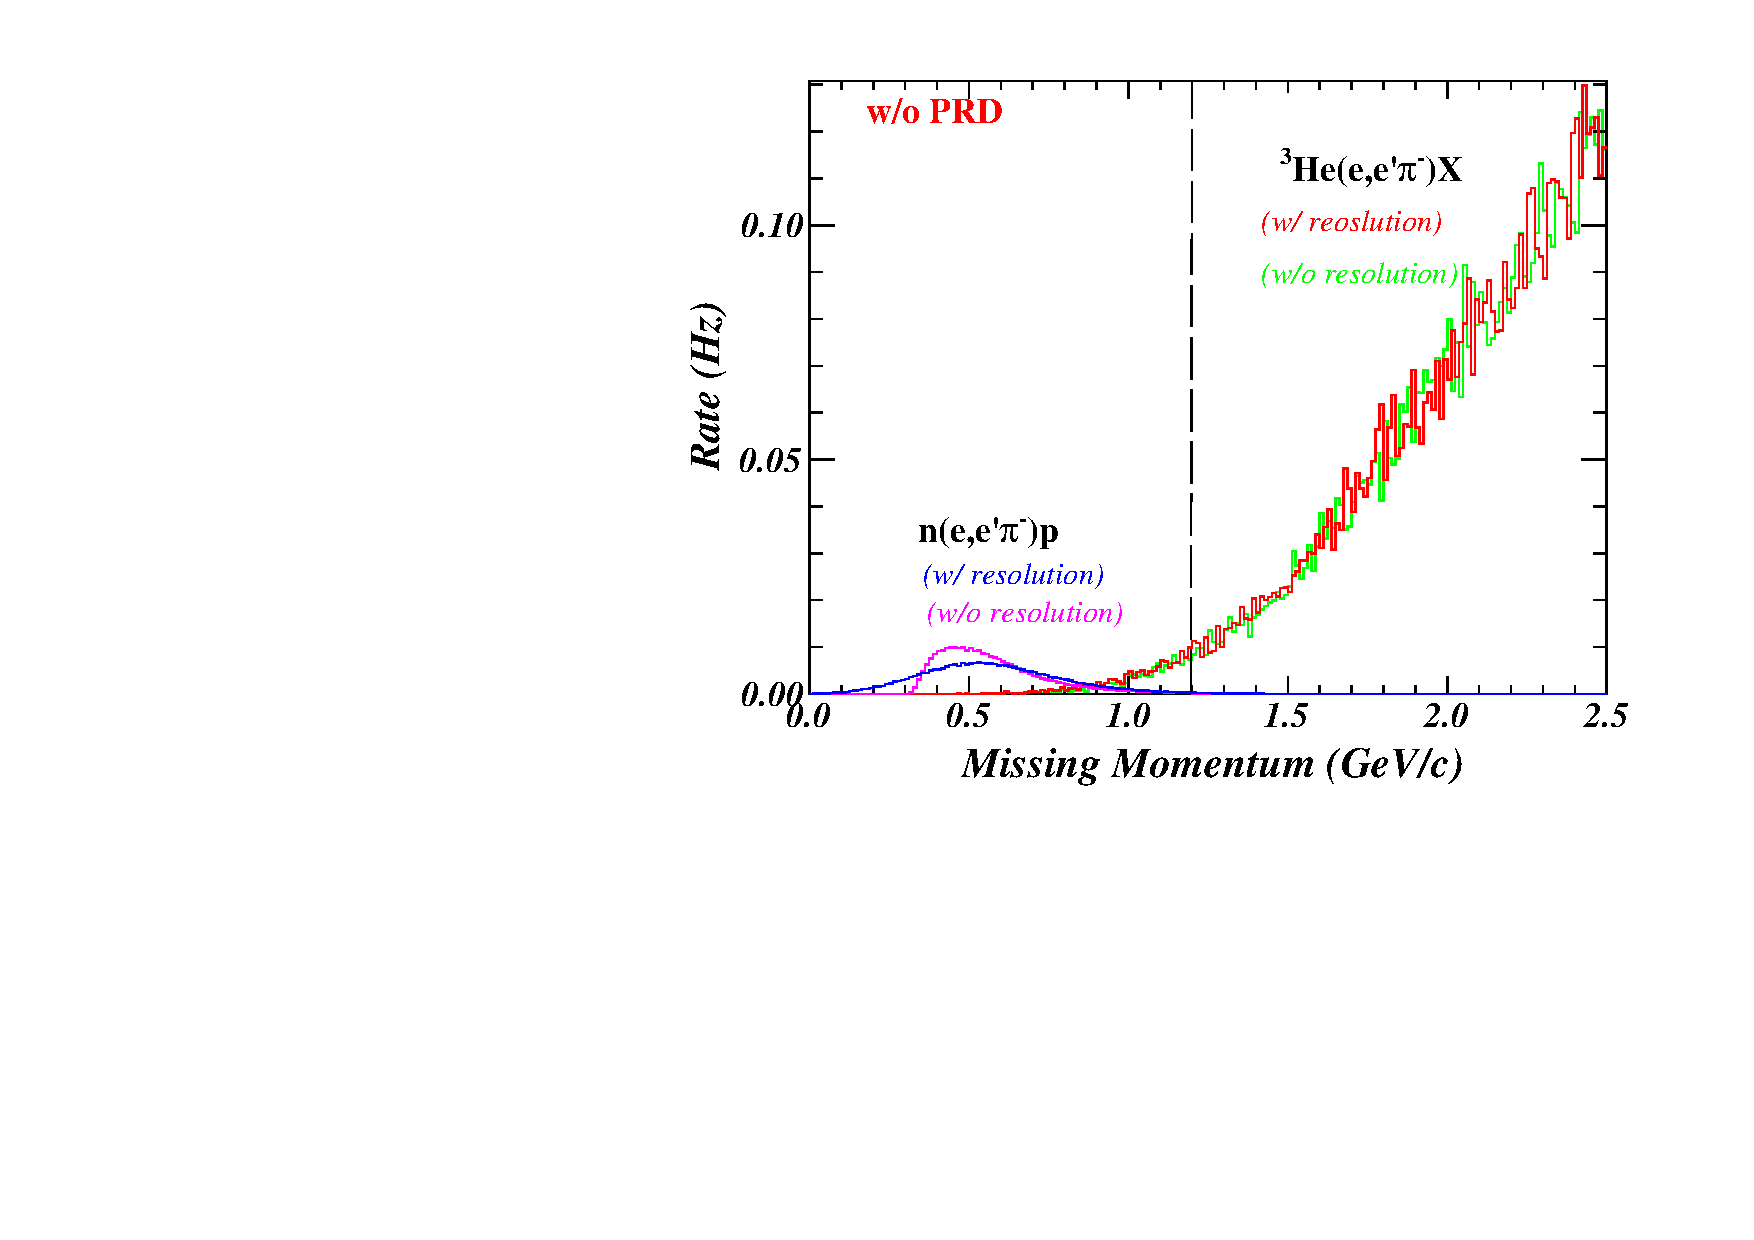
\includegraphics[type=pdf,ext=.pdf,read=.pdf,width=0.5\textwidth]{./figures/Missing_P} }
    \subfloat[w/ PRD]{
      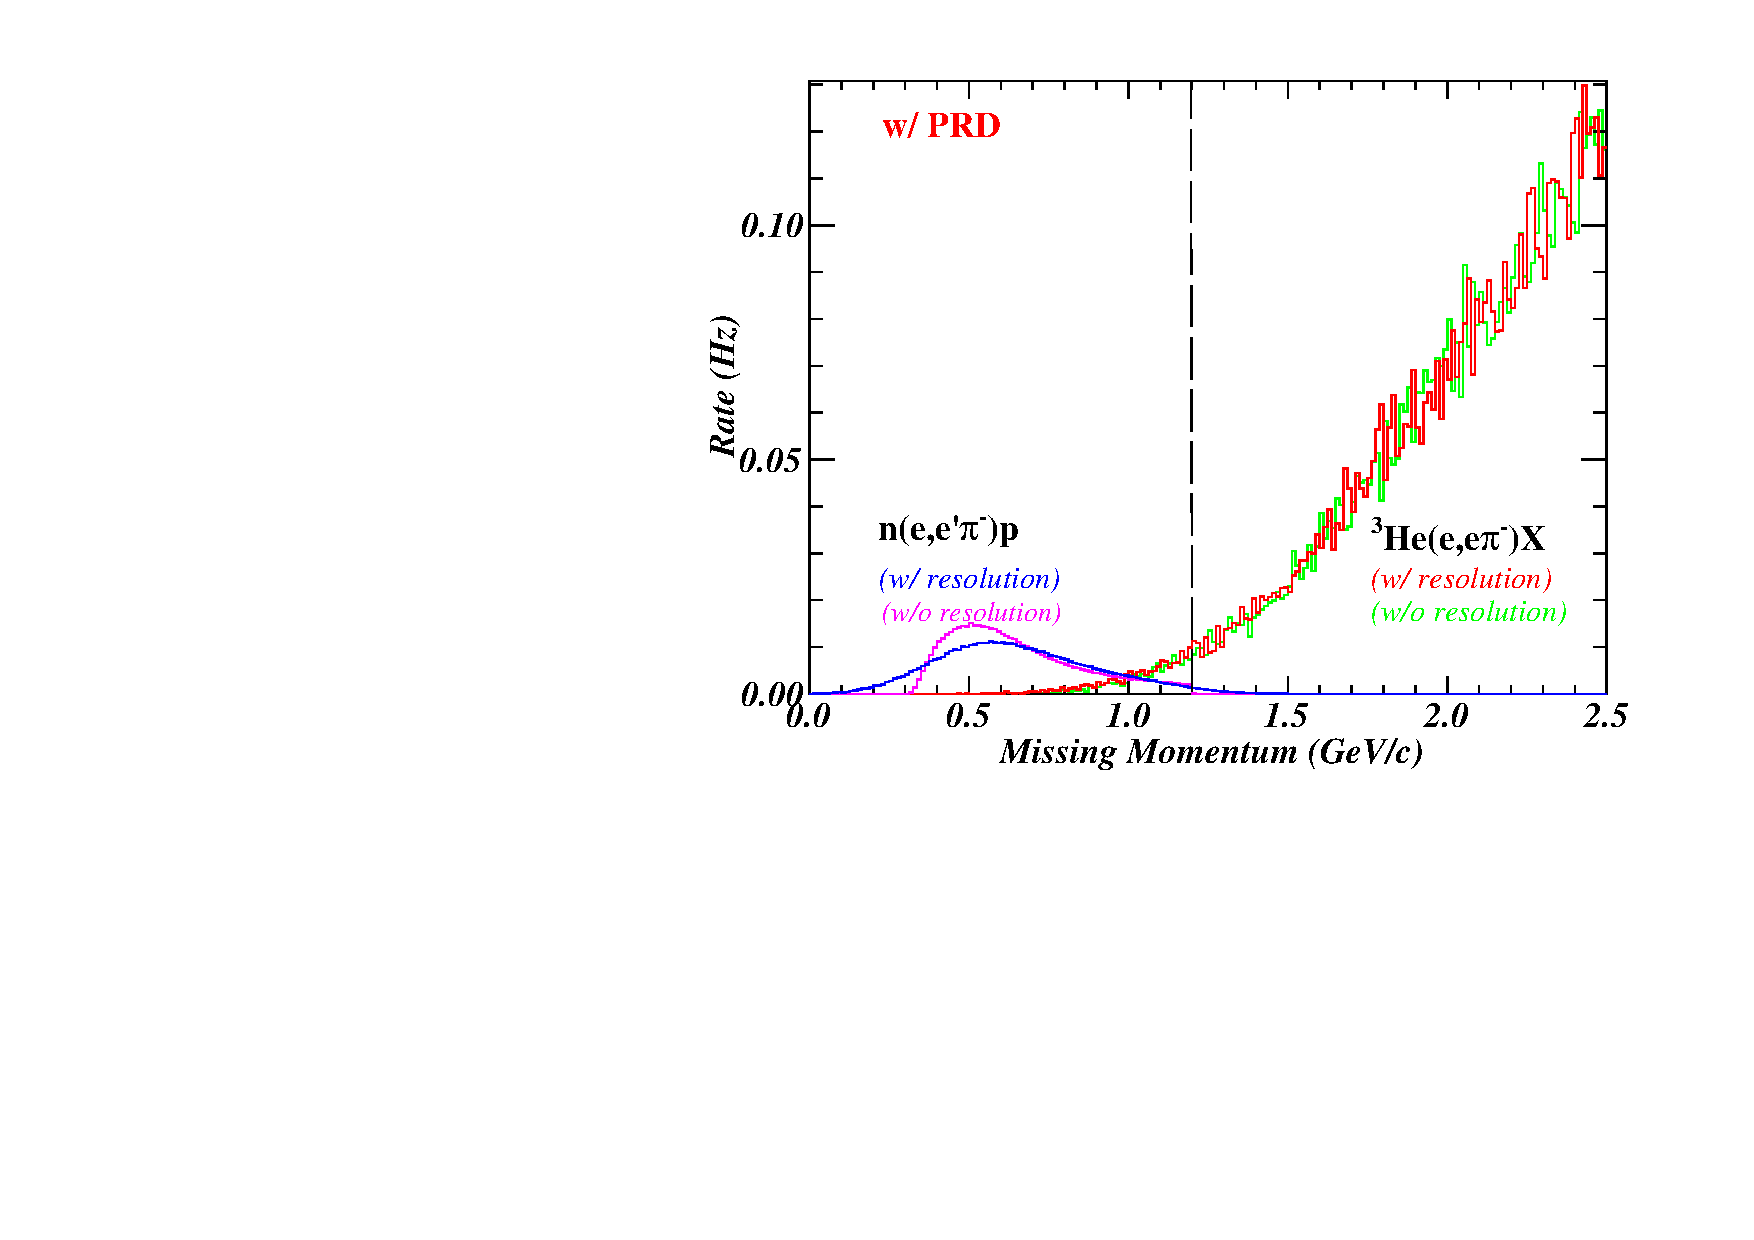
\includegraphics[type=pdf,ext=.pdf,read=.pdf,width=0.5\textwidth]{./figures/Missing_P_prd} } 
   \caption[Missing Momentum]{\footnotesize{Missing momentum spectra of DEMP and SIDIS events. The missing momentum distributes are well separated between two processes and one can apply a cut at $P_{miss}<1.2~GeV/c$ (indicated by the black dash line) to remove most of SIDIS events.}}
  \label{missing_mom}
  \end{center}
\end{figure}
Shown in Fig.~\ref{missing_mom}, we reconstruct the missing momenta of both processes. One immediately sees that the missing momentum distributions of two processes are well separated. The SIDIS background can be largely rejected when we apply a cut, $P_{miss}<1.2~GeV/c$. 

\begin{figure}[!ht]
 \begin{center}
       \subfloat[w/o PRD]{
      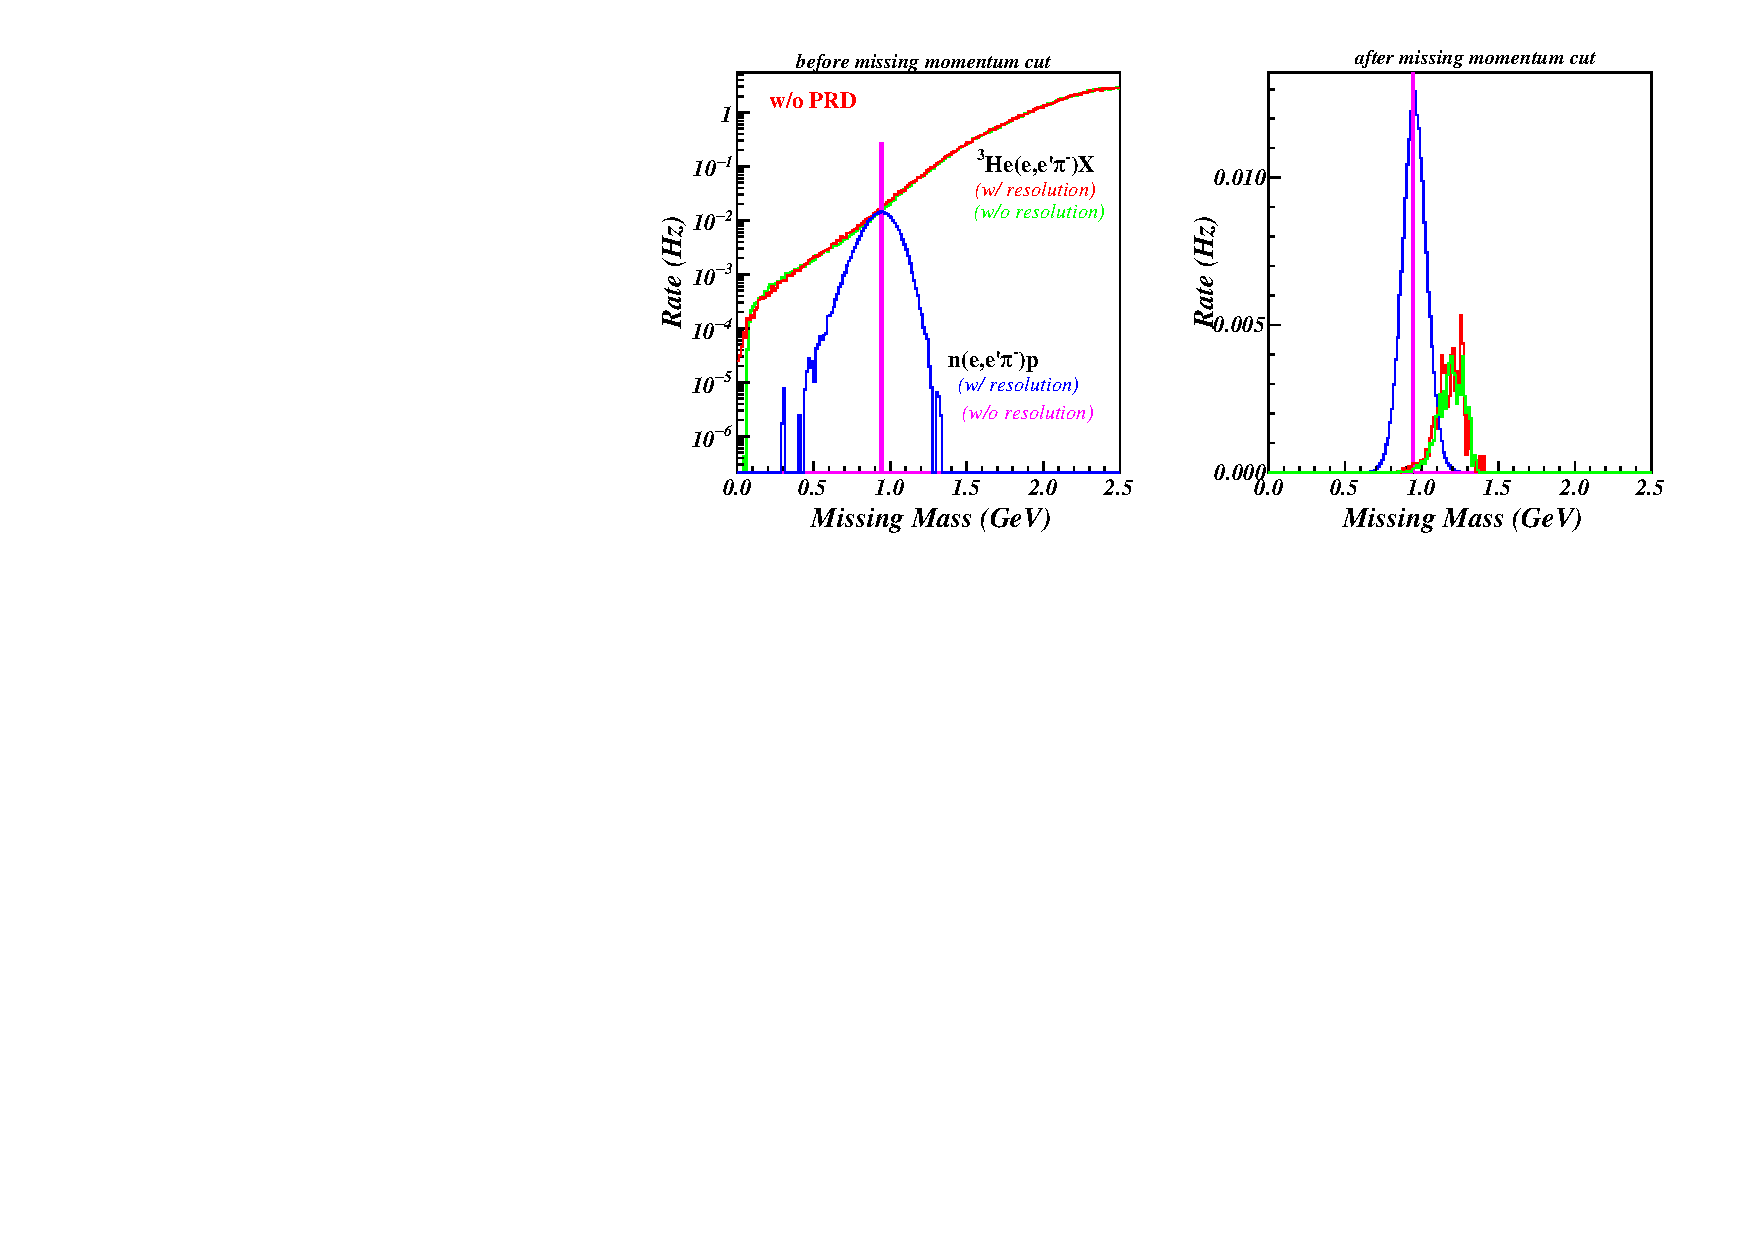
\includegraphics[type=pdf,
        ext=.pdf,read=.pdf,width=0.85\textwidth]{./figures/Missing_Mass} }\\
          \subfloat[w/ PRD]{
      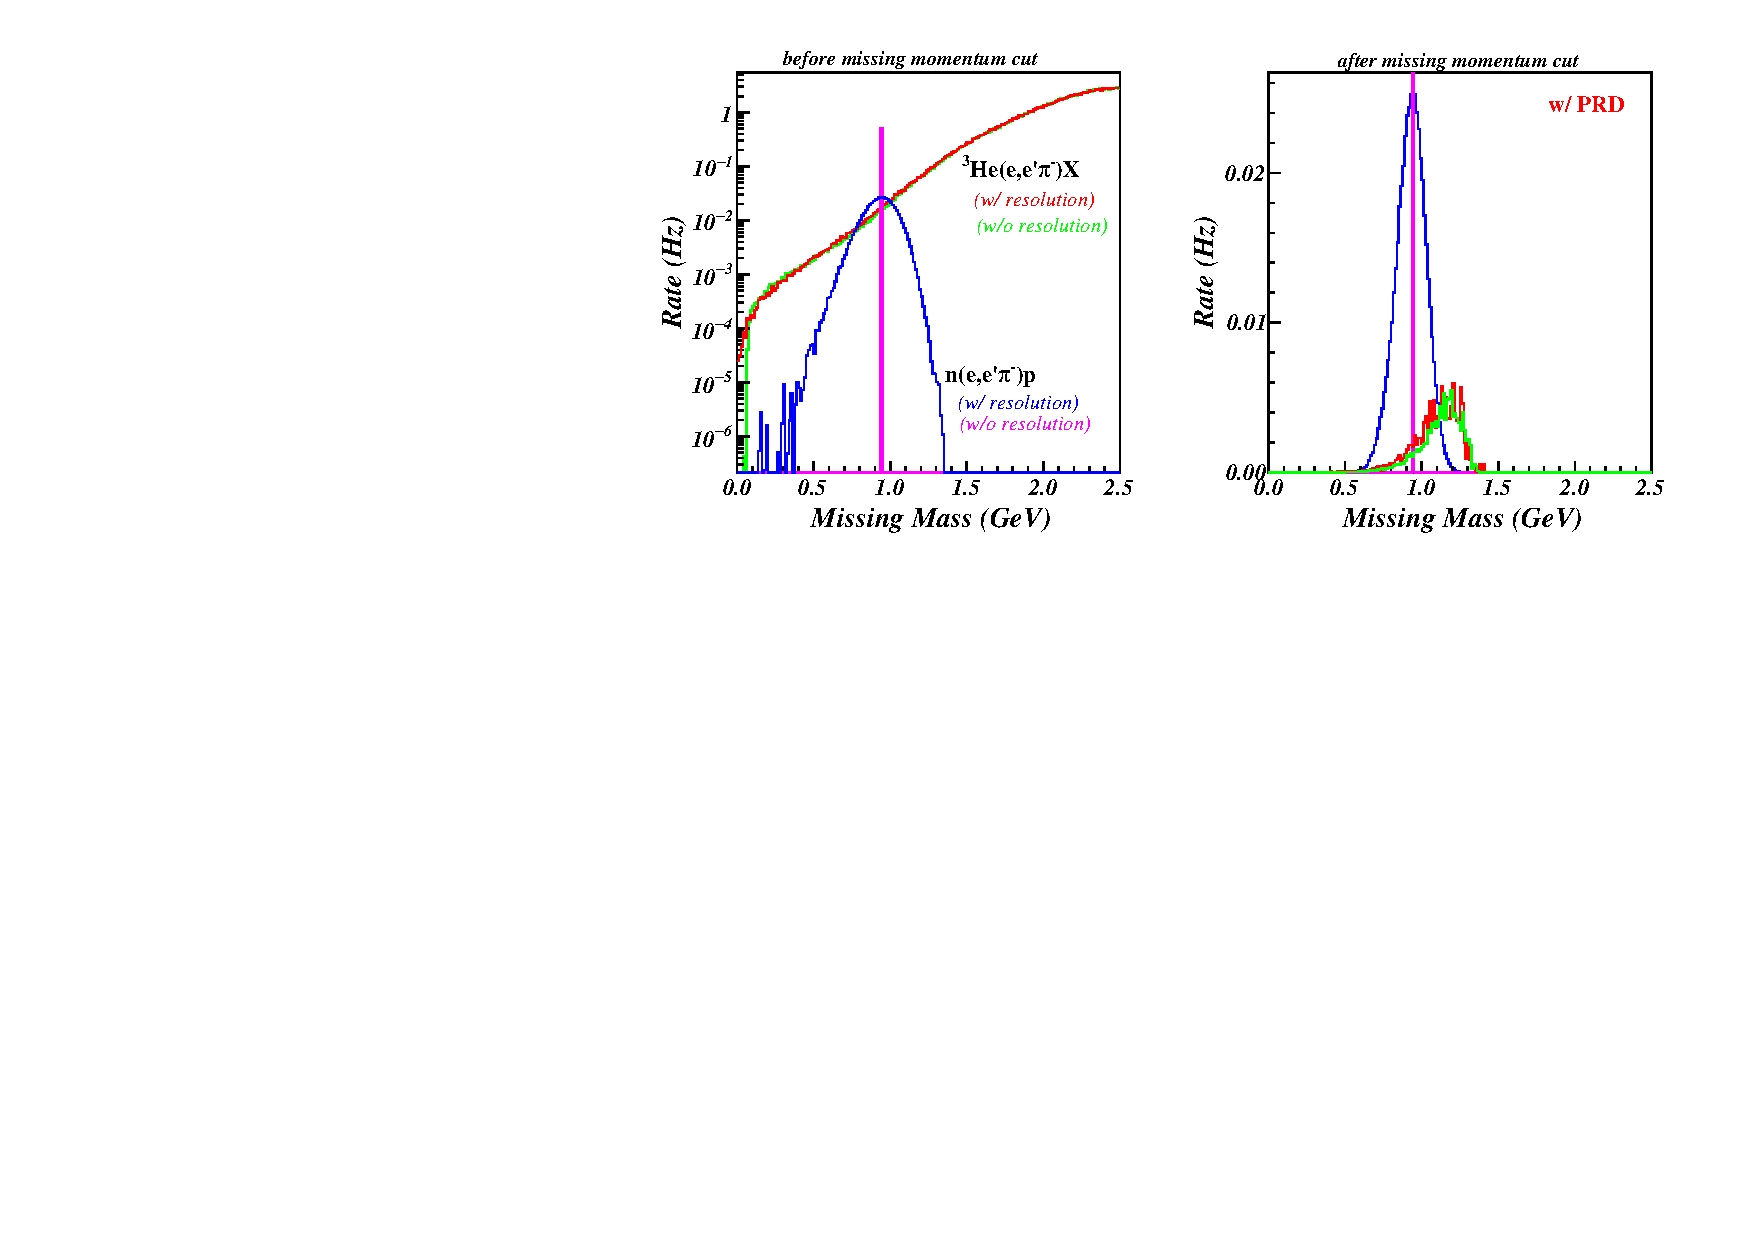
\includegraphics[type=pdf,
        ext=.pdf,read=.pdf,width=0.85\textwidth]{./figures/Missing_Mass_prd} } 
   \caption[Missing Mass]{\footnotesize{Missing mass spectra of DEMP and SIDIS events. Top (bottom) panel shows the missing mass distribution of DEMP events w/o (w/) proton detection by a new PRD. The left (right) plot of each panel shows the background contamination from SIDIS events before (after) the missing momentum cut shown in Fig.~\ref{missing_mom}. The SIDIS background is already small compared with DEMP events. The actual SIDIS background should be much smaller, since we overestimated the SIDIS rate by assuming all target fragments ("X") in the SIDIS process contain protons.}}
  \label{missing_mass}
  \end{center}
\end{figure}

We then reconstructed the missing mass spectra of the DEMP and SIDIS events w/
and w/o the missing momentum cuts, as shown in Fig.~\ref{missing_mass}. Before
applying the missing momentum cut, the SIDIS background overwhelms the DEMP
peak (note that the SIDIS rate is likely overestimated). After applying the
cut, the DEMP peak dominates and the SIDIS background is largely suppressed. If
we consider the fact that not every $``X''$ in SIDIS contains a proton, the
remaining background should be negligible.

Other random coincident background events will show up in the missing mass spectrum with more uniform distributions. We should be able to suppress most of them with tight missing momentum and missing mass cuts, and for these residuals that contaminate the real events, we are able to evaluate their asymmetries if nonzero, and apply corrections on the real asymmetry values. In general, we expect to have a clean measurement of the DEMP process because of all final particles being detected.


\section{Systematic Uncertainties}
\begin{table}[!htp]
\centering
\begin{tabular}{|c|c|}
\hline
{\bf Sources}            & {\bf Relative Value} \\\hline
Beam Polarization        & $2\%$ \\\hline 
Target Polarization      & $3\%$ \\\hline 
Acceptance               & $3\%$ \\\hline
Other Contamination      & $<5\%$ \\\hline
Radiation Correction     & $1\%$ \\\hline
\end{tabular}
\caption{\footnotesize{Expected systematic errors.}}\label{table:det_sys_err}
\end{table}
The detector related systematic errors are expected to be similar to the ones
given in the E12-10-006 proposal as well as in other SIDIS experiments with
SoLID. Here we list several major sources of systematic uncertainties as shown
in Table~\ref{table:det_sys_err}.
